\documentclass[12pt, a4paper, onecolumn]{article}
\usepackage{fontspec}
\usepackage{titlesec}
\usepackage{tocloft}
\usepackage[english]{babel}
\usepackage{blindtext}
\usepackage{subfig}
\usepackage{pgf}
\setmainfont{Georgia}
\usepackage{parskip}
\usepackage{float}

\newcommand\sectionfont{\normalfont\fontspec{Arial}\fontsize{14pt}{0}\bfseries}
\newcommand\subsectionfont{\normalfont\fontspec{Arial}\fontsize{13pt}{0}\bfseries}
\newcommand\subsubsectionfont{\normalfont\fontspec{Arial}\fontsize{12pt}{0}\bfseries}
\newcommand\tocsectionfont{\normalfont\fontspec{Arial}\fontsize{12pt}{0}\bfseries}
\newcommand\tocsubsectionfont{\normalfont\fontspec{Arial}\fontsize{11pt}{0}\bfseries}
\newcommand\tocsubsubsectionfont{\normalfont\fontspec{Arial}\fontsize{11pt}{0}}
\newcommand\toctitlefont{\normalfont\fontspec{Arial}\fontsize{16pt}{0}\bfseries}

\titleformat{\section}{\sectionfont}{\thesection}{20pt}{}
\titleformat{\subsection}{\subsectionfont}{\thesubsection}{20pt}{}
\titleformat{\subsubsection}{\subsubsectionfont}{\thesubsubsection}{20pt}{}

\renewcommand{\cftsecfont}{\tocsectionfont}
\renewcommand{\cftsubsecfont}{\tocsubsectionfont}
\renewcommand{\cftsubsubsecfont}{\tocsubsubsectionfont}
\renewcommand{\cftsecpagefont}{\tocsectionfont}
\renewcommand{\cftsubsecpagefont}{\tocsubsectionfont}
\renewcommand{\cftsubsubsecpagefont}{\tocsubsubsectionfont}
\renewcommand{\cfttoctitlefont}{\toctitlefont}

\newcommand{\parag}[1]{
	\textbf{#1} \hspace{0pt} \\
}

\addto\captionsenglish{
	\renewcommand{\contentsname}{Table of Contents}
}

\begin{document}

\subsection{Machine learning}
Machine learning is a field within computer science dealing with methods to get computers to learn from data without specifically being programmed to do so in advance. In it´s essence, this field of research is a mixture between statistical analysis, artificial intelligence and pattern recognition. Machine learning has many sub-fields and methods, one of them is neural networks. 

\subsubsection{Structure of neural networks}
A neural network tries to mimic the human brains structure of interconnected nodes called neurons in order to make a decision based on some input \cite{mit-neural-netwirks}. A common user case for a neural network is that of classification, which means to classify something based on some input. An example could be classifying image content. Using an image containing a dog as input, the out put would thus ideally be "Dog". The network is usually structured to have an input layer, an output layer and one or several layers in between called "hidden layers". In each layer (besides the input layer) there are usually several neurons, whom each takes their input from all the neurons in the previous layer, and each send their output to all neurons in the successive layer. 

The input layer is usually a (multidimensional) vector containing the data (numerical values) to examine. In the case of classification, the output layer then has as many neurons as there are possible classes. The output is thus yet another vector with the independent probability coherence for the input to each of the classes, or in the case of one-hot-classification, a binary representation in a vector with the decided class set to one, and the other classes set to zero. 

Between the neurons in each layer are connections. Every single connection has a weight which is determined when training the neural network. Each neuron also have an activation function and a bias.
	
\newpage
	
The output of each neuron is calculated according to formula \ref{neuron-formula}:

	 \begin{equation}
	 	\label{neuron-formula}
		f((\sum_{k=1}^{n} X_{k} * W_{k}) + b)
	\end{equation}
	
where:


\begin{itemize}
	\item $n$ is the number of inputs to the neuron
	\item $X_{k}$ is the input from a single neuron in the previous layer
	\item $W_{k}$ is the weight of a single connection
	\item $b$ is the bias of the neuron
	\item $f$ is the activation function of the neuron (for example sigmoid).
\end{itemize}


There are many activation functions to choose from but a common one is the "sigmoid" function seen i \ref{sigmoid} \cite{towards-data-sci}:

\begin{equation}
\label{sigmoid}
f(x)=1/1 + e^{-x}
\end{equation}

The purpose of the activation function is to map the sum of a neuron's inputs to a value in a distinct range \textit{(0, 1), (-1, 1) etc.} in order to prepare it as input to the neurons in the next layer \cite{towards-data-sci}. 

Figure \ref{fig:neural-network-overview} illustrates a general design of a simple, densely connected, feed-forward neural network. The network has a one-dimensional vector of length three as input, and a one-dimensional vector of length two as output representing probabilities of the two output-classes. Each neuron in a previous layer is connected to all a neurons in the successive layer, and each single connection has it´s own weight. 

	\begin{figure}[H]
		\centering
		\subfloat{{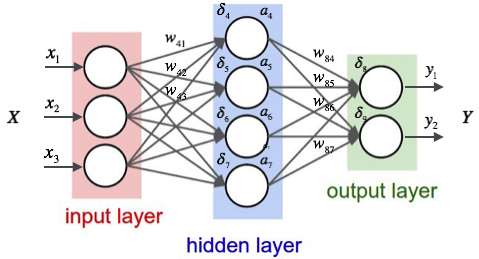
\includegraphics[width=8cm]{../img/neural-network-overview.png} }}%
		\caption{An example of a neural network with 3 features in the input layer, two neurons in the output layer and a single hidden layer with 4 neurons.}%
		\label{fig:neural-network-overview}%
	\end{figure} 
 
	\subsubsection{Training neural networks}
	When training a neural network, the individual weights are set to random values initially. All labeled training data is then fed into the network, this is called \textit{feed-forward}. At the end of each data sample feed, the output probability is compared to that particular sample's class using a loss function, the weight are then adjusted to better be able to predict the class and the process repeats. The adjustment of weights is called \textit{back-propagation}. A run through of all the samples in the training data set (feed-forward) followed by equally as many adjustments to weights (back-propagation) is called an \textit{epoch}. Training a neural network usually involves many epochs. When the network has been trained, the accuracy can be measured, using a test data set with unlabeled data \cite{neural_networks}.
	
\bibliography{bib_peter}
\bibliographystyle{ieeetr}

\end{document}